\documentclass{hw_template}

\title{\huge\sffamily\bfseries Контрольна Робота. Частина \#1}
\author{\Large\sffamily Захаров Дмитро}
\date{\sffamily 12 вересня, 2024}

\begin{document}

\pagestyle{fancy}

\maketitle

\subsection*{Умова}

Задана наступна динамічна система:

\begin{equation*}
    \begin{cases}
        \dot{x}_1 = x_1 - 2x_2 - u, \\
        \dot{x}_2 = 2x_1 - 4x_2 + 4u
    \end{cases}
\end{equation*}

\begin{enumerate}
    \item Для заданої системи перевірити умову Калмана.
    \item Для заданої системи перевірити, що не існує власного вектору матриці $A^*$, ортогонального усім стовпцям матриці $B$.
    \item Знайти матрицю керованості $N$ і довести, що вона додатно визначена або має обернену.
    \item Знайти керування, яке переводить систему з точки\footnote{Під позначенням $(x_1,\dots,x_n)$ надалі розуміємо матрицю-колонку $[x_1,\dots,x_n]^{\top}$.} $\mathbf{x}_0 = (-2,0)$ у точку $\mathbf{x}_T = \mathbf{0}$ за заданий час $T=4$.
    \item Побудувати чисельно траєкторію як параметрично задану функцію.
\end{enumerate}

\subsection*{Розв'язання}

\subsubsection*{Пункт 1}

Для цього і наступних пунктів перепишемо нашу систему у більш стандартному для нас вигляді. Отже, нехай $\mathbf{x} := (x_1,x_2)$. Тоді наша система має вигляд:
\begin{equation*}
    \dot{\mathbf{x}} = A\mathbf{x} + B\mathbf{u}, \quad A = \begin{bmatrix}
        1 & -2 \\
        2 & -4
    \end{bmatrix}, \quad B = \begin{bmatrix}
        -1 \\ 4
    \end{bmatrix}
\end{equation*}

Для перевірки умови Калмана, складемо матрицю Калмана:
\begin{equation*}
    K = \begin{bmatrix}
        B & AB & A^2B & \dots & A^{n-1}B
    \end{bmatrix},
\end{equation*}

проте в нашому випадку все дуже просто, оскільки $n=2$, і тому $K = \begin{bmatrix}
    B & AB
\end{bmatrix}$. Добуток $AB$ знайти дуже просто:
\begin{equation*}
    AB = \begin{bmatrix}
        1 & -2 \\
        2 & -4
    \end{bmatrix}\begin{bmatrix}
        -1 \\ 4
    \end{bmatrix} = \begin{bmatrix}
        1 \cdot (-1) + (-2) \cdot 4 \\
        2 \cdot (-1) + (-4) \cdot 4
    \end{bmatrix} = \begin{bmatrix}
        -9 \\ -18
    \end{bmatrix}
\end{equation*}

Тому наша матриця має вигляд:
\begin{equation*}
    K = \begin{bmatrix}
        -1 & -9 \\
        4 & -18
    \end{bmatrix}
\end{equation*}

Тепер власне згадаємо, навіщо нам ця матриця. Критерій Калмана стверджує, що система є повністю керованою на $[0,T]$ тоді і тільки тоді, коли $\text{rank}(K) = n$ ($n=2$ в нашому випадку). В цілому, це вже видно з самої матриці $K$, проте давайте все ж таки це покажемо формально. Для цього достатньо довести лінійну незалежність, скажімо, стовпців матриці. Отже, розглядаємо лінійну комбінацію $\alpha(-1, 4)+\beta(-9,-18) = (-\alpha-9\beta,4\alpha-18\beta)$. Це дорівнює нулю тоді, коли $\alpha=-9\beta$ (щоб занулити першу компоненту) і тоді для другої компоненти $(-36-18)\beta = -54\beta = 0$, звідки $\alpha=\beta=0$. Отже, стовпці матриці $K$ лінійно незалежні, що дає $\text{rank}(K) = 2$, і тому система є повністю керованою.

\subsubsection*{Пункт 2}

Спочатку знайдемо $A^*$:
\begin{equation*}
    A^* = A^{\top} = \begin{bmatrix}
        1 & 2 \\
        -2 & -4
    \end{bmatrix}
\end{equation*}

Щоб знайти власні вектори цієї матриці, спочатку знайдемо власні числа з характеристичного рівняння. Для цього розглядаємо характеристичний поліном:
\begin{equation*}
    \chi_{A^*}(\lambda) = \det(A^* - \lambda E_{2 \times 2}) = \det \begin{bmatrix}
        1-\lambda & 2 \\
        -2 & -4-\lambda
    \end{bmatrix} = \lambda(\lambda+3)
\end{equation*}

Звідси одразу власні значення $\lambda_1 = 0$ і $\lambda_2 = -3$. Тепер знаходимо власні вектори. Для цього розглядаємо рівняння $A^*\mathbf{v} = \lambda_{j}\mathbf{v}, j \in \{1,2\}$. Маємо:
\begin{equation*}
    \begin{bmatrix}
        1 & 2 \\
        -2 & -4
    \end{bmatrix}\begin{bmatrix}
        v_1 \\ v_2
    \end{bmatrix} = \mathbf{0} \quad \text{звідки} \quad \begin{cases}
        v_1 + 2v_2 = 0, \\
        -2v_1 - 4v_2 = 0
    \end{cases}
\end{equation*}

Тому якщо покладемо $v_2 := t$, то $v_1 = -2t$ і тому маємо множину власних векторів $(-2,1)t$. Далі, для $\lambda_2=-3$ маємо:
\begin{equation*}
    \begin{bmatrix}
        1 & 2 \\
        -2 & -4
    \end{bmatrix}\begin{bmatrix}
        v_1 \\ v_2
    \end{bmatrix} = -3\begin{bmatrix}
        v_1 \\ v_2
    \end{bmatrix} \quad \text{звідки} \quad \begin{cases}
        v_1 + 2v_2 = -3v_1, \\
        -2v_1 - 4v_2 = -3v_2
    \end{cases}
\end{equation*}

Достатньо розглянути перше рівняння (оскільки друге є однаковим), звідки $2v_1+v_2=0$ і тому поклавши $v_1 := u$, маємо $v_2=-2u$. Звідси маємо інший набір векторів $(1,-2)u$. 

Отже, підсумовуючи, маємо два сімейства власних векторів (що відповідають, відповідно, власним числам $\lambda_1=0$ і $\lambda_2=-3$):
\begin{equation*}
    \mathbf{v}_1 = \begin{bmatrix}
        -2t \\ t
    \end{bmatrix}, \quad
    \mathbf{v}_2 = \begin{bmatrix}
        u \\ -2u
    \end{bmatrix}, \quad t,u \in \mathbb{R} \setminus \{0\}
\end{equation*}

Нагадаємо, що у нас $B=(-1,4)$, і нам потрібно показати, що він не ортогональний усім власним векторам. Для цього достатньо показати, що скалярні добутки $\langle B, \mathbf{v}_1 \rangle \neq 0$ і $\langle B, \mathbf{v}_2 \rangle \neq 0$. Дійсно, маємо:
\begin{gather*}
    \langle B, \mathbf{v}_1 \rangle = (-1)(-2t) + 4t = 2t+4t = 6t \neq 0, \\
    \langle B, \mathbf{v}_2 \rangle = (-1)u + 4(-2u) = -u-8u = -9u \neq 0
\end{gather*}

Отже, $B$ не ортогональний усім власним векторам матриці $A^*$.

\subsubsection*{Пункт 3}

Нагадаємо, що матриця керованості визначається як
\begin{equation*}
    N(T) = \int_0^T U(t)U^*(t)dt, \; U(t) = e^{-At}B
\end{equation*}

Зазначимо, що рахувати таку матрицю буде теоретично дуже муторно. Ми це зробимо, бо там є цікаві моменти, але далі ми наведемо програму, яка це зробить чисельно. Так чи інакше, починаємо ми з теоретичного розрахунку.

\textbf{Знаходження матричної експоненти.} Отже, спочатку нам потрібно знайти $\exp(-At)$. Для цього діагоналізуємо матрицю $A$ (ми це можемо зробити, оскільки $\lambda_1 \neq \lambda_2$):
\begin{equation*}
    A = T\Lambda T^{-1}, \quad \Lambda = \begin{bmatrix}
        -3 & 0 \\
        0 & 0
    \end{bmatrix}, \quad T = \begin{bmatrix}
        1 & 2 \\
        2 & 1
    \end{bmatrix}, \quad P^{-1} = \frac{1}{3}\begin{bmatrix}
        -1 & 2 \\
        2 & -1
    \end{bmatrix}
\end{equation*}

В такому разі маємо:
\begin{equation*}
    e^{-At} = e^{-T\Lambda T^{-1}t} = \sum_{k=0}^{\infty} \frac{(-T\Lambda T^{-1}t)^k}{k!} = \sum_{k=0}^{\infty} \frac{(-1)^kt^k(T\Lambda T^{-1})^k}{k!}
\end{equation*}

Тепер помічаємо, що $(T\Lambda T^{-1})^k = T\Lambda^k T^{-1}$ і тому
\begin{equation*}
    e^{-At} = \sum_{k=0}^{\infty} \frac{(-1)^kt^kT\Lambda^k T^{-1}}{k!} = T\left(\sum_{k=0}^{\infty} \frac{(-1)^k t^k\Lambda^k}{k!}\right)T^{-1}
\end{equation*}

Сума в дужках рахується тепер дуже просто:
\begin{equation*}
    \sum_{k=0}^{\infty} \frac{(-1)^k t^k\Lambda^k}{k!} = E_{2 \times 2} + \sum_{k=1}^{\infty} \frac{(-1)^kt^k}{k!}\begin{bmatrix}
        (-3)^k & 0 \\
        0 & 0
    \end{bmatrix} = \begin{bmatrix}
        \sum_{k=0}^{\infty} \frac{3^kt^k}{k!} & 0 \\
        0 & 1
    \end{bmatrix} = \begin{bmatrix}
        e^{3t} & 0 \\
        0 & 1
    \end{bmatrix}
\end{equation*}

Отже, маємо:
\begin{equation*}
    e^{-At} = T\begin{bmatrix}
        e^{3t} & 0 \\
        0 & 1
    \end{bmatrix}T^{-1} = \frac{1}{3}\begin{bmatrix}
        1 & 2 \\
        2 & 1
    \end{bmatrix}\begin{bmatrix}
        e^{3t} & 0 \\
        0 & 1
    \end{bmatrix}\begin{bmatrix}
        -1 & 2 \\
        2 & -1
    \end{bmatrix} = -\frac{1}{3}e^{3t}A + F,
\end{equation*}

де $F = \frac{1}{3}\begin{bmatrix}
    4 & -2 \\ 2 & 1
\end{bmatrix}$. Можна помітити, що $F=\frac{A}{3}+E_{2 \times 2}$, тому остаточно:
\begin{equation*}
    \boxed{e^{-At} = \frac{A}{3}(1-e^{3t}) + E_{2 \times 2}}
\end{equation*}

\textbf{Інтегрування}. Тепер, множимо це на вектор $B$, щоб отримати $U(t)$:
\begin{equation*}
    U(t) = e^{-At}B = \frac{AB}{3}(1-e^{3t}) + B
\end{equation*}

Транспонуємо це, щоб отримати $U^*(t)$:
\begin{equation*}
    U^*(t) = U^{\top} = \frac{B^{\top}A^{\top}}{3}(1-e^{3t}) + B^{\top}
\end{equation*}

Отже, тепер можемо знайти матрицю керованості:
\begin{equation*}
    N(T) = \int_0^T U(t)U^*(t)dt = \int_0^T \left(\frac{AB}{3}(1-e^{3t}) + B\right)\left(\frac{B^{\top}A^{\top}}{3}(1-e^{3t}) + B^{\top}\right)dt
\end{equation*}

Далі пропоную просто розкрити дужки:
\begin{equation*}
    N(T) = \int_0^T \left(\frac{ABB^{\top}A^{\top}}{9}(1-e^{3t})^2 + \frac{ABB^{\top}}{3}(1-e^{3t}) + \frac{BB^{\top}A^{\top}}{3}(1-e^{3t}) + BB^{\top}\right)dt
\end{equation*}

Оскільки $T=4$, то інтеграл виходить так собі через доданки з $e^{3t}$. А саме:
\begin{align*}
    \gamma := & \int_0^T \frac{1-e^{3t}}{3} = \frac{13-e^{12}}{9} \approx -6.027 \times 10^3, \\
    \delta := & \int_0^{T} \frac{(1-e^{3t})^2}{9} = \frac{e^{24}-4e^{12}+27}{54} \approx 4.905 \times 10^8
\end{align*}

В такому разі маємо:
\begin{equation*}
    N(T) = ABB^{\top}A^{\top}\delta + ABB^{\top}\gamma + BB^{\top}A^{\top}\gamma + 4BB^{\top}
\end{equation*}

Цей вираз дуже неприємний. Але, можна скористатися тим, що $\delta$ на 5 порядків більший за $\gamma$ та значно більший за коефіцієнти всіх матриць. Тому, наближено (ми це потім чисельно перевіримо), можна вважати
\begin{equation*}
    N(T) \approx \hat{N}(T) = ABB^{\top}A^{\top}\delta = \delta VV^{\top} \; \text{для} \; V = AB
\end{equation*}

Матриця $VV^{\top}$ є додатно визначеною\footnote{взагалі кажучи, напівдодатно визначеною, але в нашому випадку вона додатно визначена.}, тому і $\hat{N}(T)$ додатно визначена. Звичайно, сторого кажучи, звідси не випливає, що і $N(T)$ є додатно визначеною, тому давайте проведемо все те саме, але чисельно.

\textbf{Чисельний розрахунок.} Для цього скористаємося наступним кодом:
\begin{lstlisting}[language=Mathematica]
A = {{1, -2}, {2, -4}};
B = {{-1}, {4}};
t1 = 4;
U[t_] = MatrixExp[-A*t].B;
ControlMatrix[T_] = Integrate[U[t].Transpose[U[t]], {t, 0, T}];
\end{lstlisting}

Тут через \texttt{t1} ми позначили час $T=4$. Тепер можемо знайти $N(T)$ для $T=4$:

\begin{lstlisting}[language=Mathematica]
N[ControlMatrix[t1]]

> {{3.97324*10^10, 7.94657*10^10}, {7.94657*10^10, 1.58933*10^11}}
\end{lstlisting}

Також, одразу можемо порівняти з нашою оцінкою $\hat{N}(T)$:
\begin{lstlisting}[language=Mathematica]
d[T_] = Integrate[(1-Exp[3*t])^2/9, {t, 0, T}];
PredictedControlMatrix[T_] = d[T]*A.B.Transpose[B].Transpose[A];
N[PredictedControlMatrix[t1]]

> {{3.97327*10^10, 7.94654*10^10}, {7.94654*10^10, 1.58931*10^11}}
\end{lstlisting}

Для цікавості, можемо вивести відносне відхилення. Для цього покладемо це відхилення як $\varepsilon := \|N - \hat{N}\| \big/ \|N\|$. Тоді матимемо:
\begin{lstlisting}[language=Mathematica]
e = N[Norm[ControlMatrix[t1]-PredictedControlMatrix[t1]] / Norm[ControlMatrix[t1]]]

> 0.0000132869
\end{lstlisting}

Як бачимо, воно доволі мале. Тепер щоб показати, що матриця $N(T)$ має обернену, можемо використати наступний код:
\begin{lstlisting}[language=Mathematica]
InverseControlMatrix[T_] = Inverse[ControlMatrix[T]];
N[InverseControlMatrix[t1]]

> {{0.033333, -0.0166663}, {-0.0166663, 0.00833304}}
\end{lstlisting}

На здивування, доволі простий вираз. Отже матриця керованості дійсно має обернену. Окрім того, додатну визначеність можемо побачити з критерію Сильвестра. Дійсно, верхній лівий елемент та визначник додатний. Це можна побачити з наступного коду:
\begin{lstlisting}[language=Mathematica]
D1 = N[ControlMatrix[t1][[1]][[1]]];
D2 = N[Det[ControlMatrix[t1]]];
positiveDefinite = (D1 > 0) && (D2 > 0)

> True
\end{lstlisting}

\subsubsection*{Пункт 4}

Для знаходження керування, яке переводить систему з точки $\mathbf{x}_0 = (-2,0)$ у точку $\mathbf{x}_T = \mathbf{0}$ за час $T=4$, можемо скористатися формулою:
\begin{equation*}
    \mathbf{u}(t) = U^*(t)N^{-1}(T)\left(e^{-AT}\mathbf{x}_T - \mathbf{x}_0\right)
\end{equation*}

Оскільки в нас $\mathbf{x}_T = \mathbf{0}$, то це спрощується до
\begin{equation*}
    \mathbf{u}(t) = -U^*(t)N^{-1}(T)\mathbf{x}_0
\end{equation*}

Вирази страшні, тому рахуємо чисельно:
\begin{lstlisting}[language=Mathematica]
x0 = {{-2}, {0}};
u[t_] = -Transpose[U[t]].InverseControlMatrix[t1].x0;
u[t_] = Simplify[u[t][[1]][[1]]];
\end{lstlisting}

Якщо вивести $u(t)$, то вийде вираз $u(t)=\alpha(\beta-30e^{3t}+6e^{3(4+t)})$ для $\alpha \approx 2.51 \times 10^{-12}, \beta \approx -7.95 \times 10^{10}$, але звичайно, що аналітично це тягати ми не будемо. 

\subsection*{Пункт 5}

Тепер наш порахований $u(t)$ підставимо у систему рівнянь, щоб отримати траєкторію. Для цього скористаємося наступним кодом:
\begin{lstlisting}[language=Mathematica]
solution = DSolve[{x1'[t] == x1[t] - 2*x2[t] - u[t], x2'[t] == 2*x1[t] - 4*x2[t] + 4*u[t], x1[0] == -2, x2[0] == 0}, {x1[t], x2[t]}, t];
x1[t_] = solution[[1]][[1]][[2]];
x2[t_] = solution[[1]][[2]][[2]];
\end{lstlisting}

Результативні аналітичні функції $x_1(t),x_2(t)$ дуже об'ємні, але наведені у прикріпленому коді. Тепер давайте побудуємо графік траєкторії:
\begin{lstlisting}[language=Mathematica]
trajectory[t_] = Evaluate[{x1[t], x2[t]} /. solution];

Show[
    ParametricPlot[trajectory[t], {t, 0, 4}, PlotStyle -> Directive[Blue, Thickness[0.005]]] /. Line[x_] :> {Arrowheads[{0., 0.05, 0.05, 0.05, 0.}], Arrow[x]}, 
    ListPlot[{Labeled[{-2, 0}, "x_0"], Labeled[{0, 0}, "x_T"]}, 
    PlotStyle -> Directive[Blue, PointSize[0.02]], 
    LabelStyle -> {20, Bold}],
    GridLines -> Automatic,
    ImageSize -> 600,
    AxesLabel -> {"x_1", "x_2"},
    LabelStyle -> {14, FontFamily},
    AxesStyle -> Arrowheads[{0.0, 0.05}],
    PlotRange -> {{-2.5, 0.5}, {-1.5, 0.5}}
]
\end{lstlisting}

Отримуємо Рисунок~\ref{fig:trajectory}.

\begin{figure}[H]
    \centering
    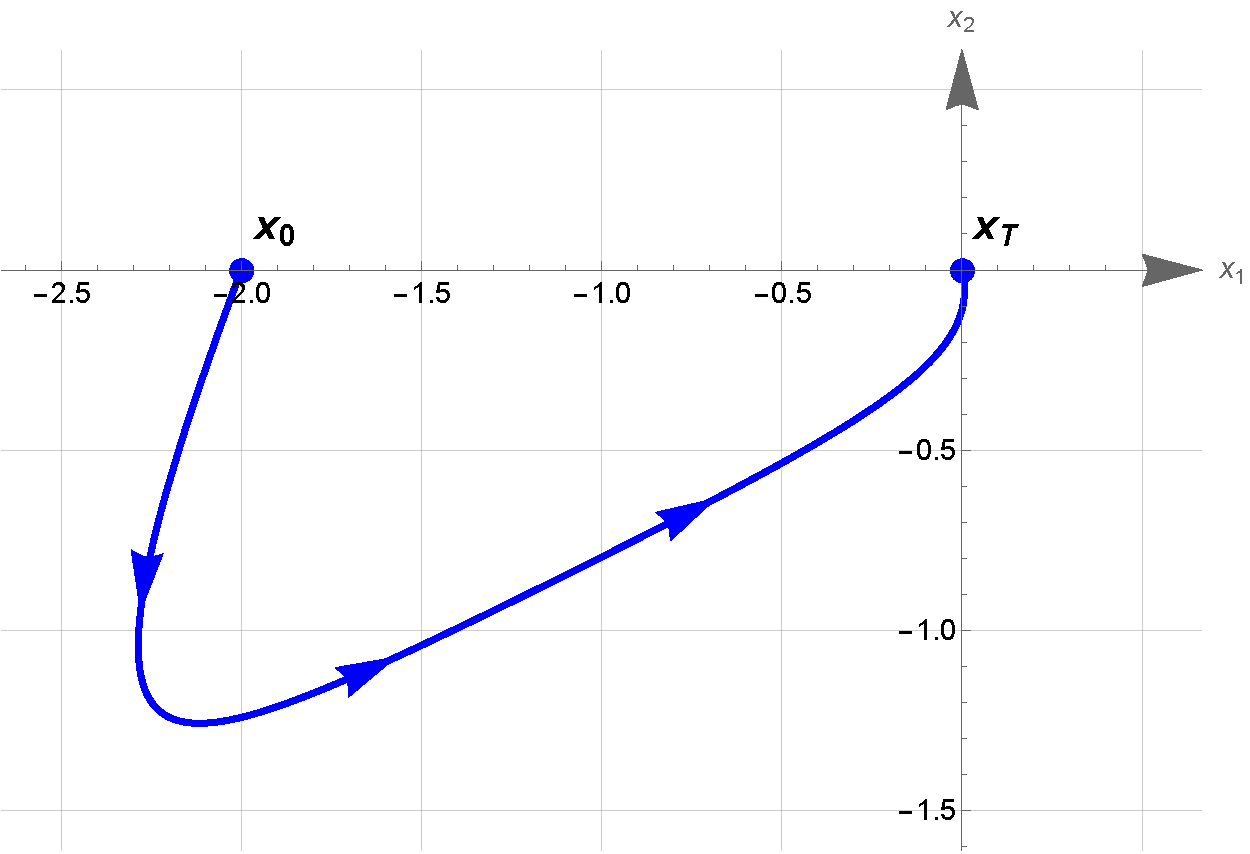
\includegraphics[width=0.7\textwidth]{figures/homework_1.pdf}
    \caption{Траєкторія системи}
    \label{fig:trajectory}
\end{figure}

\end{document}